\chapter{Experimental setup}

The thin foil stacked-target technique was applied to measure the experimental cross sections for reactions induced in iridium, iron, nickel and copper with deuteron energies ranging from ca. 33-5 MeV. This method is well-described in literature \footnote{https://sci-hub.tw/https://doi.org/10.1016/j.nimb.2016.09.018}\footnote{Niobium paper and iron paper from Andrew} for protons. This is however the first experiment using deuterons and the results may differ as for instance the deuteron break up effect is unknown. 

\section{Lawrence Berkeley National Laboratory's 88" Cyclotron}

Lawrence Berkeley National Laboratory (LBNL) is a national research laboratory on behalf of the U.S. Department of Energy through its Office of Science, and is operated by University of California, Berkeley. LBNL was founded by Ernest Orlando Lawrence, the inventor of the cyclotron \footnote{https://www.lbl.gov/about/}. \\ 


\noindent
The 88" Cyclotron has many purposes, and can accelerate both light and heavy ions up to Uranium, with a cyclotron number K=140  \footnote{http://cyclotron.lbl.gov/home}. %The cyclotron number is the maximum kinetic energy which can be reached for protons (with no relativistic factors taken into account). The maximum kinetic energy a particle can gain is found from the cyclotron number:

%\begin{equation}
%    \frac{E_k}{A}=K\Big(\frac{Q}{A}\Big)^2
%\end{equation}
\noindent 
%For deuterons with mass number A=2 and charge Q=1, the maximum kinetic energy is $E_k=70$ MeV. 
There are multiple programs that takes place in the facility\footnote{https://ieeexplore.ieee.org/abstract/document/7999622/authors#authors}; chip testing and space effects testing, super heavy element searches, fundamental nuclear structure measurements, novel scintillation characterization, fission yield and neutron inelastic scattering measurements (GENESIS) (from Andrew). \\

\noindent 
A cyclotron is a device that accelerates positively charged particles. It is operated by an alternating electric field, and a perpendicular magnetic field, which by the Lorentz Force forces the particle to accelerate in an outward spiral. 
The facility is figured in figure \ref{fig:LBNL_88}, which consists of a cyclotron vault, and experimental caves in which the beam can be bent to with bending magnets. Faraday cups (not in figure) can measure the beam current at different steps along the tube, which makes it possible to measure the transition efficiency of the beam. Faraday cups are dense metal block, usually 6-7 cm broad Copper and Tantilum. It works as a beam stopper, and can be lowered into the beam line to measure the current. It is electrically isolated, which makes it possible to measure the current, since we know the number of initial particles accelerated. Due to electrons close to surface might be scattered of, it can read of higher positive charge than what is correct. Therefor, a magnet surrounds the cup to bend the electrons back to the Faraday cup in what is called magnetic suppression. Cave 0 is used mainly for neutron beam, chemistry, and isotope production, and was used for irradiation of the target stack.


\begin{figure}
    \centering
    \includegraphics[width=0.8\textwidth]{Experiment/LBL_88.png}
    \caption{An overview of the 88" Cyclotron facility. https://cpb-us-e1.wpmucdn.com/sites.usc.edu/dist/7/89/files/2018/04/133-18q03um.pdf }
    \label{fig:LBNL_88}
\end{figure}

\section{The experiment}
The main motivation of this experiment was to measure production cross sections of the products produced after irradiation of a stack of thin iridium foils along with thin monitor foils Nickel, Cupper and Iron foils, with a 33 MeV incident deuteron beam, as shown in figure \ref{fig:experiment_illustration}. 
\begin{figure}
    \centering
    \includegraphics[width=0.7\textwidth]{Experiment/Illustration_beamOnTarget.png}
    \caption{The fundamental idea of the experiment where a stack of targets are placed in a target holder, and irradiated with accelerated 33 MeV deuterons. As the energy degrades through the beam stack, it is possible to have multiple cross section measurements at different energies.}
    \label{fig:experiment_illustration}
\end{figure}

The beam was ca. 1 cm in diameter, and with each target foil being ca. 25 by 25 mm, the beam was underfilled. As the energy was degraded through the stack, multiple cross sections at different energies were possible to measure for the different induced reactions. For production cross section data experiments, thin targets (foils) are used, in the other of a few $\mu$m \footnote{(Syed M. Qaim. Nuclear data for production and medical application of radionuclides:
Present status and future needs. Nuclear Medicine and Biology, 44:31–49, jan 2017.)} are used, since the induced activity is low, meaning that the deadtime of the detector and the dose to human will be low.  

\noindent 
%From equation \ref{eq:activity_eob}, the cross section as a function of energy is 

%\begin{equation} \label{eq:experimental_CS}
%    \sigma(E)=\frac{A_0}{N_T \Phi (1-e^{-\lambda \Delta t_\text{irr}})}
%\end{equation}

\noindent 
%where E is the average energy across the foil (MeV), $A_0$ is the end of beam activity (Bq), $N_T$ is the number of target nuclei, $\Phi$ is the beam current (nA), $\lambda$ is the decay constant of the nucleus ($s^{-1}$) and $\Delta t_\text{irr}$ is the irradiation length (s). 

\noindent 
Equation \ref{eq:cross_section_equation} is the equation which is used in the calculation of the cross sections. In order to calculate the cross section of a product, end of beam activity, number of target nuclei and beam current must be found, where for the end of beam activity, the detector efficiency need to be estimated. The number of target nuclei was estimated through characterization of the foils. $A_0$ was estimated using equation \ref{eq:Final_Expression_A0}, which depends on the efficiency calibration of the detectors as a function of gamma-ray energy, the number of counts registered and the intensity of the gamma-rays emitted by the source, the decay constant of the source and the delay time. Some of the nickel, copper and iron deuteron-induced cross section are well-established, and can  be used to determine the beam current throughout the stack. 



%The end of beam activity goes into the equation, which is given in equation \ref{eq:Final_Expression_A}. The activity from spectra measured at different delay times after end of beam can be found, with respect to number of counts, efficiency of detector, intensity of gamma-rays, the decay constant of the nucleus $\lambda$ and the counting time $\Delta t_c$. As we know that radioactive decay curves follows equation \ref{eq:ndecay_chains}, and dependent on how many step the decaychain consists of, the end of beam activity can be estimated by extrapolating backwards in time with a curve fit. \\

%\noindent 


\subsection{Target design and foil characterization}
\textcolor{red}{why was the order what it was??}
In this experiment, the target stack was composed of of ten natural iridium foils (99.9\%) foils, along with ten natural nickel foils (..\%), ten natural copper foils (..\%) and three natural iron foils (..\%) (from Goodfellow Corporation, Corapolis, PA 15108, USA) serving as monitor foils. Along with two stainless steel foils in the front and the back of the stack, a proton degrader (a 6061 aluminum alloy), and an extra nickel neutron monitor foil was used to obtain production cross sections at multiple energies, using one incident deuteron beam. The full order of the stack and the characterization of each foil can be seen in table \ref{table:foil_characterization}. \\

\noindent 
Each foil were cut into approximately 25 by 25 mm squares, and each foil was characterized using a caliper (Mitutoyo Absolute Digimatic) to measure the length across each side, a gauge caliper (Mitutoyo IP65 Coolant Proof) to measure the thickness and an analytical balance weight (Mettler Toledo) to measure the mass of each foil which was prewashed with isopropanol. For each measurement, the unit was measured 4 times, and the values listed in table \ref{table:foil_characterization} are averaged values. The length and mass were used to measure the mass density. The thickness was not used in the
calculation of the mass density, but was a good indication that the foil thicknesses were consistent.
\textcolor{red}{For underfilled beams, the mass density of the foil is used to find the number of nuclei per cm$^2$, by using the area of each foil.} The mass density was calculated using the mass of each foil divided by the area
\begin{equation}
    \rho \Delta r = \frac{m}{A}
\end{equation}

\noindent 
The uncertainty in each parameter was calculated using the standard deviation (equation \ref{eq:standard_dev}) of the four measurements per unit, and the total uncertainty was calculated using the approximation of uncorrelated variables used in equation \ref{eq:uncertainty_simplification}. The conversion from mg per cm$^2$ to nuclei per cm$^2$ was done numerically, by multiplying the mass density with Avogadro's number $N_A$ and dividing by the mol-mass of the target atoms. \\

\noindent 
After the characterization, each foil was mounted on a plastic frame with an open space in the middle and attached with capton tape along the edges (from previous experiments, capton tape have shown to be be a large \textcolor{red}{proton?} degrader, so it was important that the tape was not in the beamline \textcolor{red}{cite Article by Andrew}). The target frames can be seen in figure \ref{fig:targets_on_frame}. 

\begin{figure}
    \centering
    \includegraphics[width=0.5\textwidth]{Experiment/targets_on_frame.JPG}
    \caption{The figure shows the four different targets mounted on plastic frames with capton tape attached along the edges of the foils.}
    \label{fig:targets_on_frame}
\end{figure}


\begin{table}[h!]
%\centering
\caption{Characterization of each foil, along with calculated mass density. Each length is measured in mm, and mass in grams. }
\label{table:foil_characterization}
\small
\begin{tabular}{lllllll}
\makecell{\textbf{Foil}} & \makecell{Length1 (mm)}  &  \makecell{Length2 (mm)} & \makecell{Thickness (mm)} & \makecell{Mass (g)} & \makecell{\textbf{Mass density (mg/cm$^2$)}} \\ 
\hline
\makecell{SS1} & \makecell{} & \makecell{} & \makecell{} & \makecell{} & \makecell{\textbf{...}} \\
\hline
\makecell{Ni01} & \makecell{25.228} & \makecell{25.293} & \makecell{0.0285} & \makecell{0.1453} & \makecell{22.772 $\pm$ 0.138} \\
\makecell{Ir01} & \makecell{24.943} & \makecell{24.968} & \makecell{0.0295} & \makecell{0.3436} & \makecell{55.174 $\pm$ 0.053} \\
\makecell{Cu01} & \makecell{25.553} & \makecell{24.883} & \makecell{0.0341} & \makecell{0.1420} & \makecell{22.338 $\pm$ 0.048} \\
\makecell{Fe01} & \makecell{24.400} & \makecell{26.068} & \makecell{0.0278} & \makecell{0.1274} & \makecell{20.030 $\pm$ 0.110} \\
\hline
\makecell{Ni02} & \makecell{25.288} & \makecell{25.428} & \makecell{0.0295} & \makecell{0.1487} & \makecell{23.118 $\pm$ 0.096} \\
\makecell{Ir02} & \makecell{24.923} & \makecell{25.005} & \makecell{0.0278} & \makecell{0.3465} & \makecell{55.601 $\pm$ 0.238} \\
\makecell{Cu02} & \makecell{25.443} & \makecell{25.550} & \makecell{0.0348} & \makecell{0.1451} & \makecell{22.325 $\pm$ 0.028} \\
\makecell{Fe02} & \makecell{25.525} & \makecell{23.800} & \makecell{0.0274} & \makecell{0.1216} & \makecell{20.017 $\pm$ 0.034} \\
\hline
\makecell{Ni03} & \makecell{25.295} & \makecell{25.210} & \makecell{0.0270} & \makecell{0.1425} & \makecell{22.338 $\pm$ 0.066} \\
\makecell{Ir03} & \makecell{24.885} & \makecell{24.983} & \makecell{0.0243} & \makecell{0.3459} & \makecell{55.643 $\pm$ 0.121} \\
\makecell{Cu03} & \makecell{25.560} & \makecell{25.508} & \makecell{0.0343} & \makecell{0.1455} & \makecell{22.313 $\pm$ 0.043} \\
\makecell{Fe03} & \makecell{26.113} & \makecell{25.235} & \makecell{0.0310} & \makecell{0.1315} & \makecell{19.948 $\pm$ 0.114} \\
\hline
\makecell{Ni04} & \makecell{25.303} & \makecell{24.888} & \makecell{0.0273} & \makecell{0.1304} & \makecell{20.704 $\pm$ 0.068} \\
\makecell{Ir04} & \makecell{24.960} & \makecell{24.833} & \makecell{0.0261} & \makecell{0.3471} & \makecell{56.000 $\pm$ 0.109} \\
\makecell{Cu04} & \makecell{25.153} & \makecell{25.603} & \makecell{0.0333} & \makecell{0.1435} & \makecell{22.284 $\pm$ 0.027} \\
\hline
\makecell{Ni05} & \makecell{25.325} & \makecell{25.495} & \makecell{0.0263} & \makecell{0.1406} & \makecell{21.768 $\pm$ 0.045} \\
\makecell{Ir05} & \makecell{24.948} & \makecell{24.958} & \makecell{0.0256} & \makecell{0.3435} & \makecell{55.161 $\pm$ 0.081} \\
\makecell{Cu05} & \makecell{25.213} & \makecell{25.573} & \makecell{0.0334} & \makecell{0.1447} & \makecell{22.443 $\pm$ 0.028} \\
\hline
\makecell{Ni06} & \makecell{25.530} & \makecell{25.195} & \makecell{0.0285} & \makecell{0.1471} & \makecell{22.861 $\pm$ 0.123} \\
\makecell{Ir06} & \makecell{24.760} & \makecell{24.960} & 
\makecell{0.0240} & \makecell{0.3444} & \makecell{55.731 $\pm$ 0.088} \\
\makecell{Cu06} & \makecell{25.343} & \makecell{25.513} & \makecell{0.0340} & \makecell{0.1448} & \makecell{22.396 $\pm$ 0.012} \\
\hline
\makecell{Ni07} & \makecell{25.338} & \makecell{25.278} & \makecell{0.0268} & \makecell{0.1479} & \makecell{23.092 $\pm$ 0.078} \\
\makecell{Ir07} & \makecell{24.955} & \makecell{25.008} & \makecell{0.0278} & \makecell{0.3538} & \makecell{56.685 $\pm$ 0.085} \\
\makecell{Cu07} & \makecell{25.625} & \makecell{25.248} & \makecell{0.0326} & \makecell{0.1444} & \makecell{22.320 $\pm$ 0.014} \\
\hline
\makecell{Ni08} & \makecell{25.205} & \makecell{24.950} & \makecell{0.0256} & \makecell{0.1409} & \makecell{22.409 $\pm$ 0.124} \\
\makecell{Ir08} & \makecell{24.723} & \makecell{24.985} & \makecell{0.0281} & \makecell{0.3585} & \makecell{58.030 $\pm$ 0.130} \\
\makecell{Cu08} & \makecell{25.370} & \makecell{24.885} & \makecell{0.0333} & \makecell{0.1414} & \makecell{22.401 $\pm$ 0.033} \\
\hline
\makecell{Ni09} & \makecell{25.220} & \makecell{25.378} & \makecell{0.0257} & \makecell{0.1392} & \makecell{21.741 $\pm$ 0.073} \\
\makecell{Ir09} & \makecell{24.670} & \makecell{24.993} & \makecell{0.0273} & \makecell{0.3494} & \makecell{56.669 $\pm$ 0.043} \\
\makecell{Cu09} & \makecell{25.390} & \makecell{26.455} & \makecell{0.0331} & \makecell{0.1506} & \makecell{22.425 $\pm$ 0.041} \\
\hline
\makecell{Ni10} & \makecell{25.285} & \makecell{24.405} & \makecell{0.0271} & \makecell{0.1425} & \makecell{23.093 $\pm$ 0.024} \\
\makecell{Ir10} & \makecell{24.973} & \makecell{24.980} & \makecell{0.0270} & \makecell{0.3435} & \makecell{55.065 $\pm$ 0.055} \\
\makecell{Cu10} & \makecell{25.470} & \makecell{25.338} & \makecell{0.0355} & \makecell{0.1440} & \makecell{22.314 $\pm$ 0.047} \\
\hline


\hline
\makecell{SS2} & \makecell{} & \makecell{} & \makecell{} & \makecell{} & \makecell{\textbf{...}} \\
\makecell{P-degrader} & \makecell{} & \makecell{} & \makecell{} & \makecell{} & \makecell{\textbf{...}} \\
\makecell{Ni neutron monitor} & \makecell{} & \makecell{} & \makecell{} & \makecell{} & \makecell{\textbf{...}} \\
\hline
\end{tabular}
\end{table}


\subsection{Irradiation of target stack}
The irradiation included tuning of the beam and one hour of radiation over the target stack. Whenever the beam was turned on, the beam tube had to be pumped down to a vacuum, to not attenuate the beam. The target holder was a 6061 aluminum alloy with a hole in the front for the beam. The targetholder was placed in the end of the beam tube (\textcolor{red}{mounts of the end of an electrically-isolated beamline, (iron paper andrew)}). The targetholder can be visualized in figure \ref{fig:targetstack}, with a spring holding the foils stable (\ref{fig:stack}a) and placed in the end of the beam tube (\ref{fig:stack}b). 

\subsubsection{Tuning the beam}
The cyclotron was tuned for a 33 MeV deuteron beam, and needed to have the correct beam spot. First, the beam spot was visualized using a ca. 2.5 cm thick borosilicate glass, painted with a mixture of phosphor powder and vacuum grease (so that the paint does not evaporate as the tube was pumped down to vacuum). When ionizing radiation strikes the phosphor, the phosphor is excited and emits light in the de-excitation, called phosphorescence.  The glass is placed on the end of the beam tube. With a camera placed in cave 0, from the control room, the beam spot could be visualized, and could be steered to be centered and ca. 1 cm in diameter. Secondly, visualization of the beam throughout the beam stack was important to see that the beam did not diverge converge/diverge or move in the wrong direction over the target stack. Gafchromic films which change color if struck by ionizing radiation was placed in the front and the back of the target holder, separated by the spring. The films were exposed for a brief second, and the blue spot was evaluated. This was done until the beamspot was good both in the front and in the back of the stack. \\

\noindent
The beam efficiency transmission was calculated by measuring the the current at the Faraday cup right after the cyclotron vault (BS-02) and right before cave 0 (FC-01). BS-02 was measured to be 420 nA and FC-01 was measured to be 285 nA. This gave beam efficiency of transmission

$$\frac{FC-01}{BS-02}=67\% $$

\subsubsection{Irradiation of the target stack}

The targetstack was irradiated for exactly an hour, and the current was read of the beam integrator evenly, to assure that the it increased constantly. The beamcurrent from the beam integrator read 128.5 nA.  %The full scale ameperes was $2\cdot 10^{-7}$A.
Right after end of beam, the targets were sealed in plastic bags to avoid contamination. The foils were counted at the seven different detectors for the following 4 weeks after end of beam, first short counts to get as many observations as possible of the short-lived activities and longer and longer counts as the times since end of beam passes, so that the counting statistics for the longer lived activites are good. 

\begin{figure}%
    \centering
    \subfloat[The target stack in target holder]{{\includegraphics[width=6.6cm]{Experiment/stack.JPG} }}%
    \subfloat[Target holder placed in the end of beam tube]{{\includegraphics[width=6.6cm]{Experiment/tube.JPG} }}%
    \caption{Figure shows the target stack and how it was placed in the beam tube.}%
    \label{fig:targetstack}%
\end{figure}


\subsubsection{Intensity profile of the beam}

After irradiation, gafchromic film were attached to the activated stainless steel in the front and the back of the stack, to obtain an intensity profile of the beam. The radius of the activity from stainless on gafchromic film is used in the imaging process program Image-J, which can be seen on figure \ref{fig:SS1_gafchromic}. The gafchromic films were scanned, and the intensity data (\textcolor{red}{x and y arrays}) were obtained by inverting the scanned image, and drawing a line segment along the beam spot that automatically created an position dependent intensity array. The intensity profile can be fitted to a Gaussian, which is shown examplewise in figure \ref{fig:beamprofile}, which is the horizontal beam profile in the front and the back of the stack. In the assumption that the beam was underfilled, it was important to build confidence in that the beamspot was ca. 1 cm in diameter, which was done estimating the full width half maximum of the Gaussian profile. The FWHM over SS1 was 1.2017 cm horizontally ($\sigma^2=$0.2604 cm$^2$) and 1.1420 cm vertically ($\sigma^2=$0.2352 cm$^2$). The FWHM over SS2 was 0.6706 cm horizontally ($\sigma^2=$0.0811 cm$^2$) and 0.5783 cm vertically ($\sigma^2=$0.0603 cm$^2$). \\

\textcolor{red}{Normally the beam broadens throughout the stack due to scattering. As we can see, this not the case, since the beam is stopped in the targetstack, and therefor we do not know how much the beam truly scatters. This gives a higher uncertainty.  
The stainless steel (which consist of ..) has fast decay time. However since it emits beta-particles, the radius will slightly increase, and the true beam spot is slightly smaller. Thus the estimated FWHM values for SS1  seems to be within the criterion for underfilled targets. }



\begin{figure}
    \centering
    \includegraphics[width=0.3\textwidth]{Experiment/gafchromic_beamprofile.jpg}
    \caption{The gafcromic film on the activated SS1 foil. }
    \label{fig:SS1_gafchromic}
\end{figure}

\begin{figure}%
    \centering
    \subfloat[Horizontal intensity profile of SS1]{{\includegraphics[width=6.6cm]{Experiment/ss_front_h.png} }}%
    
    \quad
    \subfloat[Horizontal intensity profile at SS2]{{\includegraphics[width=6.6cm]{Experiment/ss_back_h.png} }}%
    \caption{Figure shows the intensity profile of the deuteron beam in the front and in the back of the stack horizontally.}%
    \label{fig:beamprofile}%
\end{figure}


\begin{figure}
    \centering
    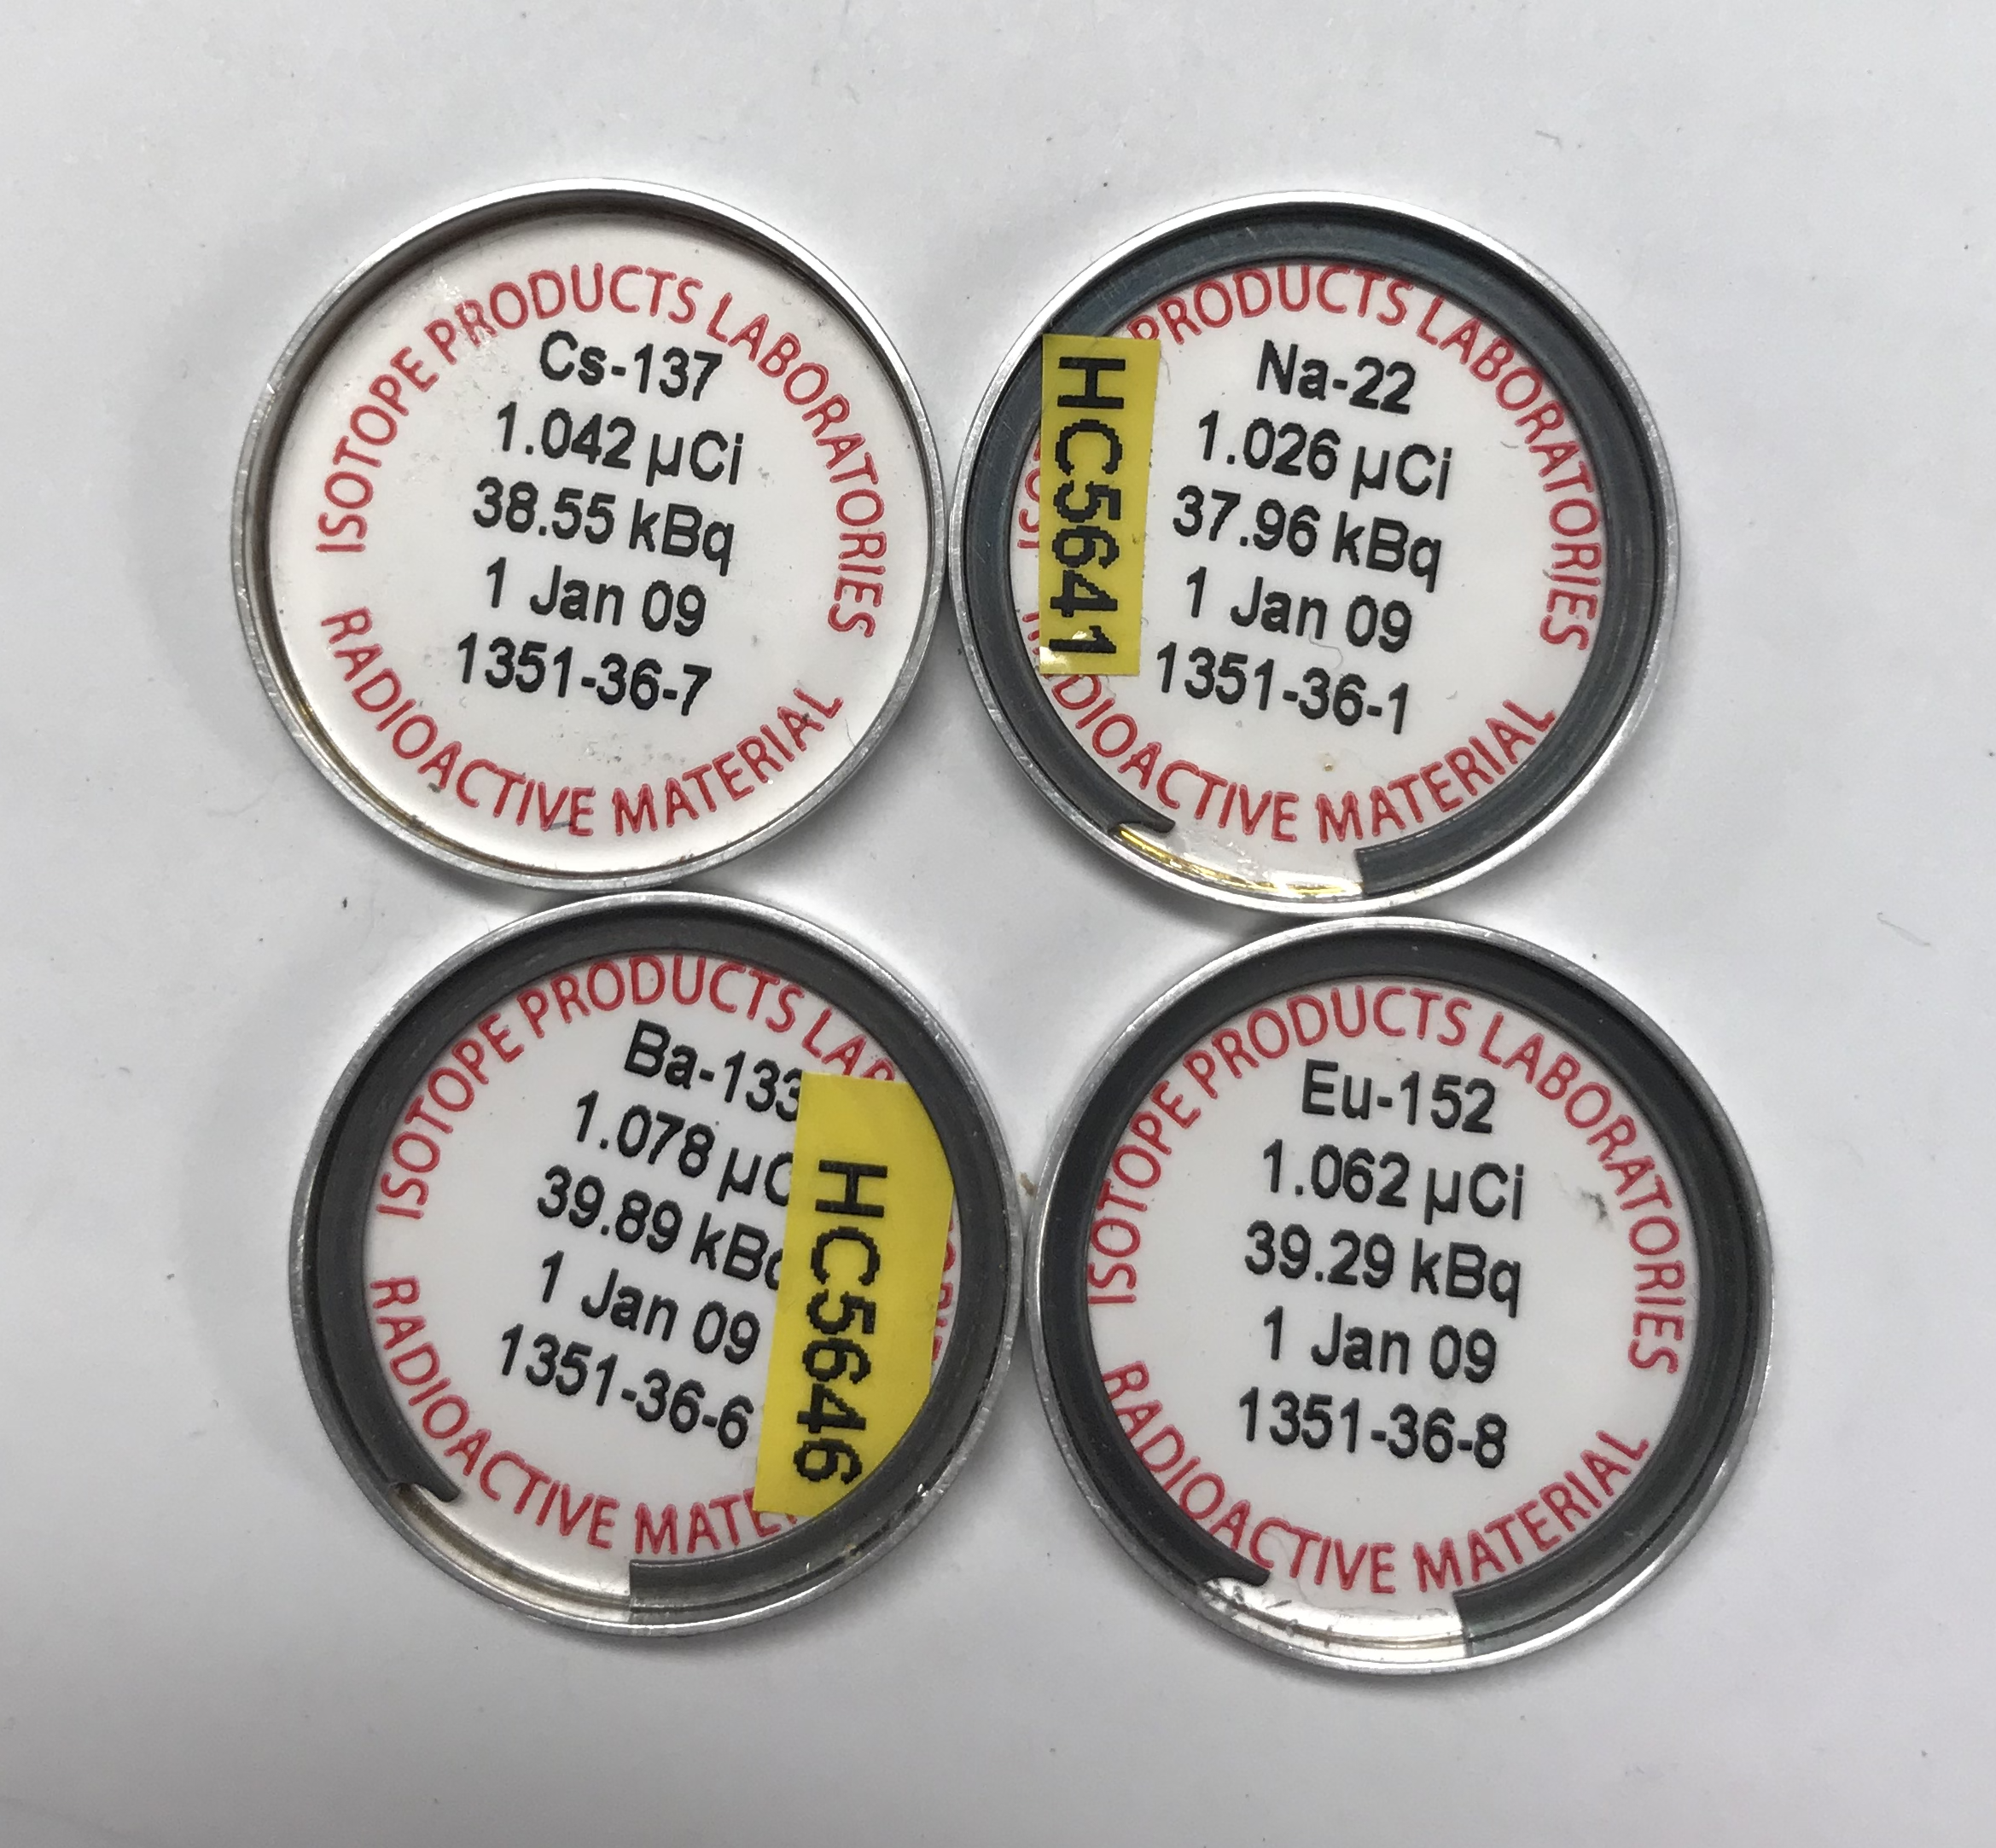
\includegraphics[width=0.5\textwidth]{Experiment/cal_sources.png}
    \caption{The calibration point sources that were used in the efficiency calibration of the detector. ($^{22}$Na was excluded because it was difficult to work with. )}
    \label{fig:calsources}
\end{figure}

\begin{table}[]
    \centering
    \caption{The calibration point sources along with gamma lines used in the calibration of the detectors. * indicates that the value has been averaged over two peaks with similar energy, less than 1 keV. For the intensity its just added together. }
    \begin{tabular}{|cc|cc|cc|}
        \hline
        
         \multicolumn{2}{|c}{\makecell{^{137}Cs}} & \multicolumn{2}{c}{\makecell{^{133}Ba}} & \multicolumn{2}{c|}{\makecell{^{152}Eu}}\\
         %\hline 
         \Xhline{2\arrayrulewidth}
         \makecell{E_\gamma}& \makecell{I_\gamma}&\makecell{E_\gamma}& \makecell{I_\gamma}& \makecell{E_\gamma}& \makecell{I_\gamma}\\
         \hline
         \makecell{32.005^*} & \makecell{5.63^*} & \makecell{53.1622} & \makecell{2.14} & \makecell{121.7817} & \makecell{28.53}\\
         
         \makecell{36.3405^*} & \makecell{1.02^*} & \makecell{80.9979} & \makecell{32.9} & \makecell{244.6979} & \makecell{7.55}\\
         
         \makecell{661.657} & \makecell{85.10} & \makecell{160.6120} & \makecell{0.638} & \makecell{295.9387} & \makecell{0.440}\\
         
          &  & \makecell{223.2368} & \makecell{0.453} & \makecell{344.2785} & \makecell{26.5}\\
         
          &  & \makecell{276.3989} & \makecell{7.16} & \makecell{367.7891} & \makecell{0.859}\\
         
          &  & \makecell{302.8508} & \makecell{18.34} & \makecell{411.1165} & \makecell{2.237}\\
          
          
          &  & \makecell{356.0129} & \makecell{62.05} & \makecell{244.4853^*} & \makecell{3.125^*}\\
          
           &  & \makecell{383.8485} & \makecell{8.94} & \makecell{503.467} & \makecell{0.1524}\\
           
           &  & \makecell{} & \makecell{} & \makecell{586.2648} & \makecell{0.455}\\
           
           &  & \makecell{} & \makecell{} & \makecell{678.623} & \makecell{0.473}\\
           &  & \makecell{} & \makecell{} & \makecell{688.670} & \makecell{0.856}\\
           
           &  & \makecell{} & \makecell{} & \makecell{719.353^*} & \makecell{0.345^*}\\
           &  & \makecell{} & \makecell{} & \makecell{778.9045} & \makecell{12.93}\\
           &  & \makecell{} & \makecell{} & \makecell{810.451} & \makecell{0.317}\\
           &  & \makecell{} & \makecell{} & \makecell{867.380} & \makecell{4.23}\\
           &  & \makecell{} & \makecell{} & \makecell{963.712^*} & \makecell{14.65^*}\\
           &  & \makecell{} & \makecell{} & \makecell{1112.076} & \makecell{13.67}\\
           &  & \makecell{} & \makecell{} & \makecell{1212.948} & \makecell{1.415}\\
           &  & \makecell{} & \makecell{} & \makecell{1299.142} & \makecell{1.633}\\
           &  & \makecell{} & \makecell{} & \makecell{1408.013} & \makecell{20.87}\\
        %\makecell{^{137}Cs} & \makecell{^{133}Ba} & \makecell{^{152}Eu} \\
        \hline 
   
        \hline
    \end{tabular}
    \label{table:calibration_gammas}
\end{table}


\begin{comment}
\begin{table}[]
    \centering
    \caption{Table shows the geometry of the different detectors. }
    \begin{tabular}{|c|c|c|}
        \hline\textbf{}
        Detector & Geometry & Dimension \\
        \hline 
        \makecell{Detector 1} & \makecell{..} & \makecell{..} \\
        \makecell{Detector 1} & \makecell{..} & \makecell{..} \\      
        \makecell{Detector 3} & \makecell{..} & \makecell{..} \\     
        \makecell{Detector 4} & \makecell{..} & \makecell{..} \\  
        \makecell{Detector 5} & \makecell{..} & \makecell{..} \\    
        \makecell{Detector 6} & \makecell{..} & \makecell{..} \\      
        \makecell{Detector 7} & \makecell{..} & \makecell{..} \\     
        \hline
    \end{tabular}
    \label{tab:detector_characteristics}
\end{table}
\end{comment}


\subsection{Counting on high purity detectors}

\noindent 
Seven different detectors were used, six IDM Ortec detectors (detectors 1-6) with detector diameter 85 mm, detector length 30 mm and hole depth 15 mm, and one Germanium detector (detector 7) with detector diameter 64.9 mm, detector length 57.8 mm and hole depth 48.6 mm \textcolor{red}{from detector diagrams}. Besides, IDM detectors were located in cave 4c (see figure \ref{fig:LBNL_88}), which have previously been used as radiation chamber. Thus, background radiation was present. For detector 7, there was led shielding around the detector. Spectra taken on the Germanium detector is preferred. In order to visualize the signal from the detector, Maestro  (Multichannel Analyzer Emulation Software\footnote{https://www.ortec-online.com/products/application-software/maestro-mca}) was used. \\ 

\noindent 
The detectors were calibrated for efficiency, peak shape and gamma-ray energy using $^{137}$Cs ($t_{1/2}=30.08$ years\cite{Browne2007}), $^{133}$Ba ($t_{1/2}=10.551$ years\cite{Khazov2011}) and $^{152}$Eu ($t_{1/2}=13.517$ years\cite{Martin2013}) point sources, using the gammalines listed in table \ref{table:calibration_gammas}. The calibration was done at various distances from the detector surface. The point sources can can be seen on figure \ref{fig:calsources}. The energy and peakshape calibration was done in FitzPeakz which is described in section \ref{subsec:fitz_calibration}. The efficiency calibration is described in section \ref{sec:efficiency_calibration}. \\ 

\noindent 
The iridium foils were counted within 15 minutes after end of beam, and the other foils following up after. All the foils were counted for ca. four weeks following end of beam, with short counts in the beginning to have good statistical data for the short-lived activities, and longer and longer counts as the shorter and medium-lived activities decayed out, to have good statistics (enough counts). Since the detectors were calibrated at various distances, the deadtime of the foils right after end of beam could be reduced, however, as high as  16-22\% deadtime was present, but reduced to less than 5\% within a certain time after end of beam. 



\begin{comment}
\begin{figure}%
    \centering
    \subfloat[]{{\includegraphics[width=5cm]{Fe_56Co.png} }}%
    \quad
    \subfloat[]{{\includegraphics[width=5cm]{Ni_61Cu.png} }}%
    \subfloat[]{{\includegraphics[width=5cm]{Ni_56Co.png} }}%
    \quad
    \subfloat[]{{\includegraphics[width=5cm]{Ni_58Co.png} }}%
    \quad
    \subfloat[caption]{{\includegraphics[width=5cm]{Cu_62Zn.png} }}%
    \quad
    \subfloat[]{{\includegraphics[width=5cm]{Cu_63Zn.png} }}%
    \quad
    \subfloat[]{{\includegraphics[width=5cm]{Cu_65Zn.png} }}%
    \quad
    \caption{Figure shows the estimation of monitor cross section using the calculated beam current. It is compared along with the monitor data.  }%
    \label{fig:monitor_BC}%
\end{figure}

\end{comment}